% Sec. Link Instrumentation
\section{Link Instrumentation}
\label{sec:link}
This section answers what the testbed observes of each link, how
often, and within what limits. Fig.~\ref{fig:linktrace} shows one run.
\todo{Extend the figure with RTT and CSI amplitude against time
alongside the agents' positions.}

\subsection{Link State}
Passive metrics are read at \SI{5}{\hertz} from the kernel wireless
interface: RSSI, negotiated bitrate and MCS, transmit retries and
failures, and channel busy ratio. During outages the monitor continues
publishing with \texttt{associated=false}, so coverage gaps appear as
explicit labels and not as missing samples. Active metrics are
obtained with \texttt{iperf3} \cite{iperf3} in \SI{4}{\second} tests,
uplink and downlink separately, in survey or cooperation mode
(Sec.~\ref{sec:decisions}); in cooperation mode the measured goodput
includes the contention a deployed team would face. Latency is
measured as ICMP round-trip time at \SI{100}{\hertz}:
\SI{3.3}{\milli\second} when idle and \SIrange{60}{109}{\milli\second}
under load, the latter caused by queueing and not by path loss.
\todo{The 24 Sep passes give \SIrange{5}{10}{\milli\second} idle and
\SIrange{25}{33}{\milli\second} under iperf load; state both passes
and the load that produced each, or report the range across passes.}

\subsection{Channel State}
\label{sec:csi}
CSI is extracted with Nexmon \cite{nexmon} on a BCM43455c0 in monitor
mode at \SI{80}{\mega\hertz}, which yields one estimate over 242 used
subcarriers per received frame from its VHT-LTF. The extractor,
\texttt{sniffer}, is carried on \texttt{mobile\_1} with a
\SI{2.4}{\giga\hertz} management link kept off the measured band; it
captures the frames of \texttt{mobile\_2} and \texttt{infra\_1}. Only
QoS data frames give full-bandwidth estimates; control frames are
captured for PHY diagnosis but excluded from analysis, since mixing
them changes the effective bandwidth from frame to frame. The achieved
data-frame rates were \SI{141}{\hertz} from \texttt{infra\_1} and
\SI{104}{\hertz} from \texttt{mobile\_2}.

The channel varies over roughly half a wavelength of motion,
$\lambda/2 = \SI{26.1}{\milli\metre}$ at \SI{5745}{\mega\hertz}. If
three estimates per half-wavelength are required to follow these
variations, the achieved rates are sufficient up to a relative speed
of about \SI{1.2}{\metre\per\second}; above that the CSI is too sparse
to resolve them. The rate cannot simply be raised by sending more
packets, since Wi-Fi aggregates many packets into one transmission and
each transmission yields a single channel estimate from its preamble;
disabling aggregation would raise the CSI rate but distort the
throughput being measured. CSI phase is not coherent across devices,
which run on independent oscillators, so each transmitter--receiver
pair is treated as an independent sensing link.

\begin{figure}[t]
\centering
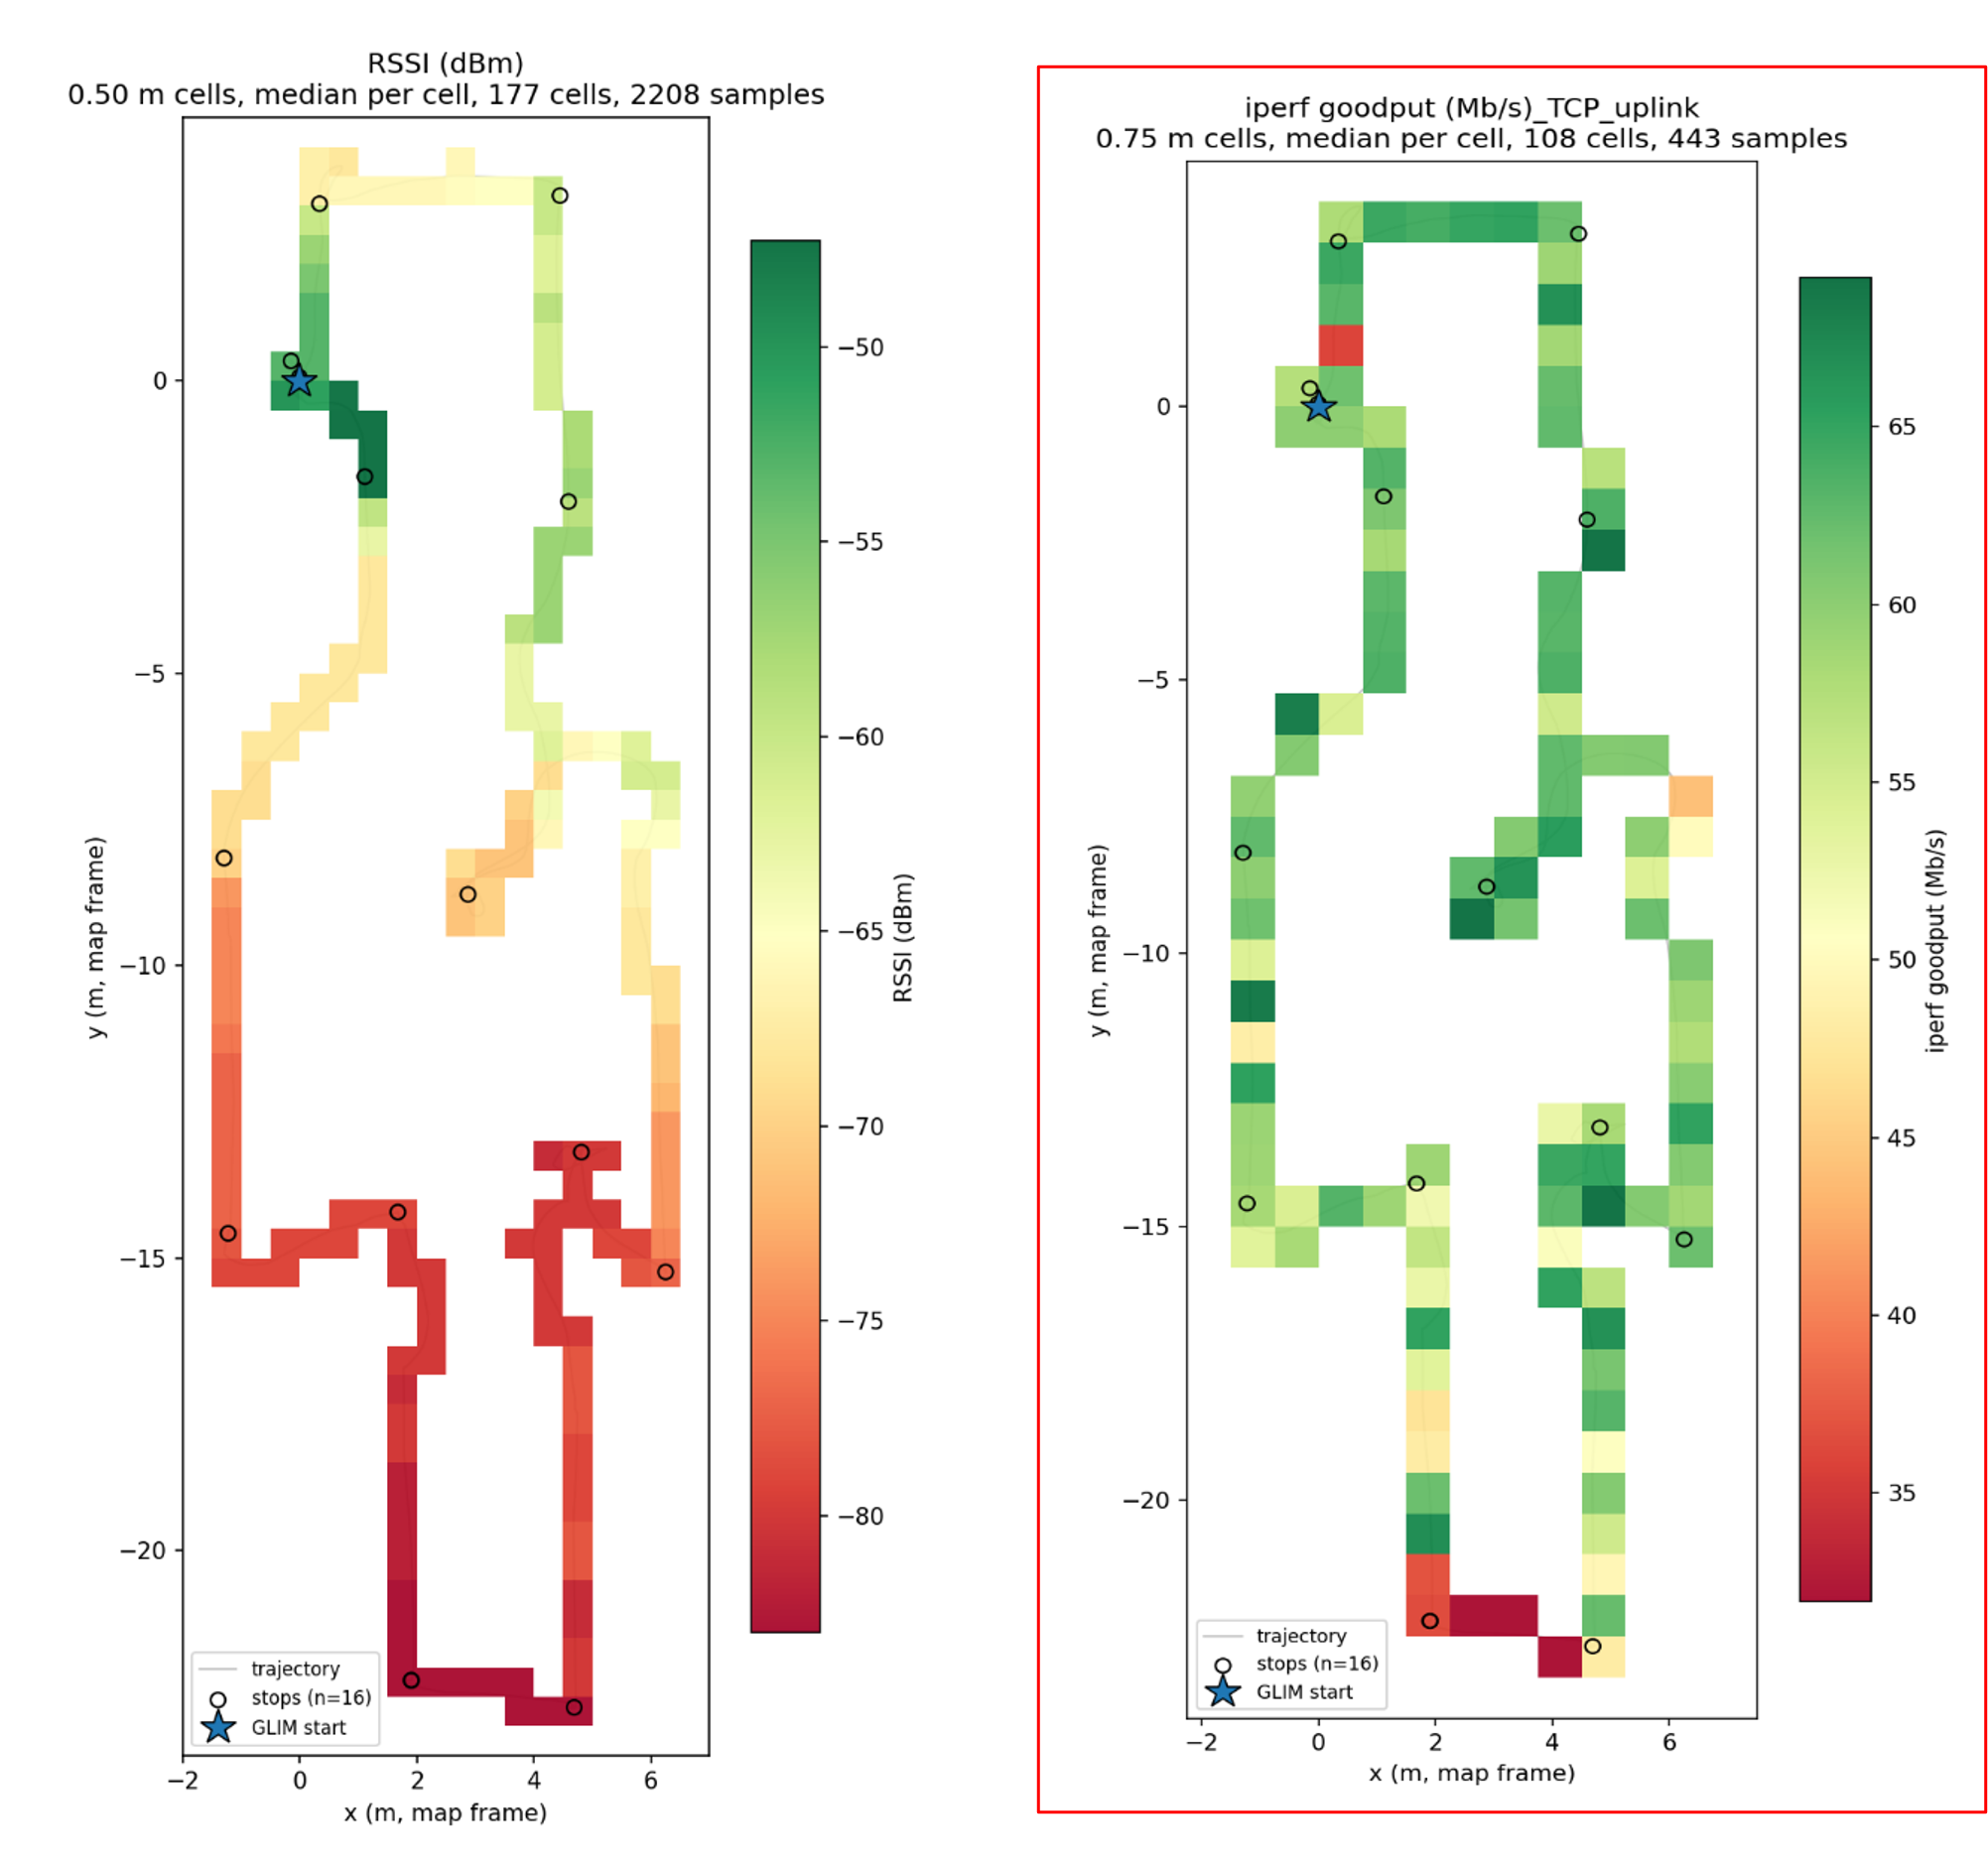
\includegraphics[width=\columnwidth]{figs/fig09_link_trace.png}
\caption{Measured link over one survey sequence at site 1, in the
reference map frame. Left: RSSI, median per \SI{0.5}{\metre} cell
(177 cells, 2208 samples). Right: TCP uplink goodput from
\texttt{iperf3}, median per \SI{0.75}{\metre} cell (108 cells, 443
samples). Circles mark the 16 survey stops, the star the start of the
mapping trajectory.}
\label{fig:linktrace}
\end{figure}

